%
% Cura.tex
%
% LulzBot Mini User Manual
%
% Copyright (C) 2014 Aleph Objects, Inc.
%
% This document is licensed under the Creative Commons Attribution 4.0
% International Public License (CC BY-SA 4.0) by Aleph Objects, Inc.
%

\section{\texttt{Cura}}
\index{Cura}
\label{Cura}

\subsection{\texttt{Setup Cura}}
\index{Installation}
Cura is available for download on our website at \texttt{https://www.LulzBot.com/cura}. When installing, it is recommended to uninstall any previous versions of Cura you may have been using. 
When first opening Cura, you will be prompted to go through the \texttt{First Run Wizard}. This will consist of selecting your printer.

\textcolor{red}{It is important to select the correct printer, as Cura uses custom profiles and machines settings based upon which printer you are running.}

\begin{itemize}
\item Download the appropriate installer for your computer operating system. Instructions on installation for each operating system is available at \texttt{http://LulzBot.com/cura}
\item Install Cura by double clicking on the installer.
%\item Once your language has been selected, select \texttt{Next}.
\item Select \texttt{LulzBot Mini}. 
\item Once the proper printer is selected, select \texttt{Next}.
\item Select which toolhead you have installed and select \texttt{Next}.
\item Select \texttt{Finish}. 
\end{itemize}

Once the installation wizard finishes you can move forward with your first print!


\section{\texttt{Quick Print Settings}}
\index{Quick Print Settings}
\begin{figure}[H]
\centering
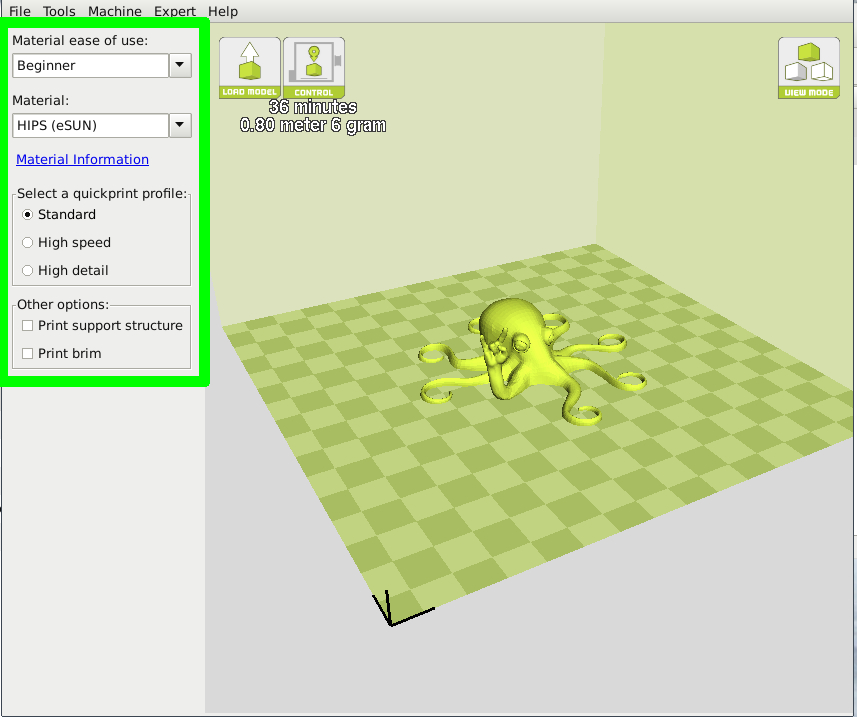
\includegraphics[keepaspectratio=true,angle=0,height=0.4\textheight,width=1.0\textwidth]{QPscreen.jpg}
\caption{Quick Print Settings}
\label{fig:Cura}
\end{figure} 
% (photo highlighting profile, material, diameter, and other)
After setting up Cura for the first time, you will be shown the main interface screen. (Fig. \ref{fig:Cura}, page \pageref{fig:Cura}): 

\subsection{\texttt{Material Selection}}
\index{Material Selection}
\index{Filament}
\index{Filament Selection}
We have the LulzBot Mini set up for 19 different types of filament straight out of the box. It is important to select the proper filament, as different filaments require different settings. We have these categorized into ease of use depending on skill level. Select \texttt{All} in order to view all 19 types of filament.
\subsection{\texttt{Selecting a Quick Print Profile}}
\index{Quick Print Profile}
\index{Resolution}
The print quality settings can be found in the top left-hand corner of the window. For most filaments, there will be Standard, High speed, or High detail options. Some of the more exotic filaments may only have a Standard profile.

\begin{description}
\item[High detail] \hfill \\
Designed to give greater detail and finer objects. This will have a smaller layer height, which will make each layer thinner, so that curves seem more natural and walls seem less noticable. This setting will also require more layers to be laid down, increasing overall print time.
\index{High detail}

\item[Standard] \hfill \\
Designed to give a medium resolution, by increasing the layer height and print speeds. This will make the organic curves slightly more step-like than the fine setting, but will reduce printing time.
\index{Standard}

\item[High speed] \hfill \\
Designed for the fast prints, where overall model finish is not of concern. Most commonly used for quick iteration of designs found in rapid prototyping.
\index{High speed}
\end{description}


%If you are not using Lulzbot supplied filament, update your filament diameter to your specific average filament diameter. Do this by taking 10 to 12 filament diameter measurements from different parts of the reel and averaging them. Update your filament diameter. %You may also want to adjust the temperature, as different manufacturers have different recommended temperatures. % This would be better served in the Full Settings explination.

\subsection{\texttt{Printing Support Material}}
\index{Support Material}
%%%% Saved for standalone Cura Manual %%%%
%The TAZ and Mini are able to print models that have angles and overhangs, even without support material depending on the overhang distance and angle. Turn this option on if your model could benefit from support material.
The LulzBot Mini 3D printer is able to print models that have angles and overhangs, even without support material depending on the overhang distance and angle. Turn this option on if your model could benefit from support material.

\subsection{\texttt{Brim}}
\index{Brim}
Brim is used to increase surface area of the part your printing, thereby ensuring proper part adhesion. This will print a single layer high edge around the outside of the part, helping first layer adhesion and minimizing warping.

\subsection{\texttt{Load Model File}}
\index{Load Model}
\index{STL}
Select the model you would like to print. Either use the \texttt{Load Model} button or select \texttt{File} > \texttt{Load Model}. Once the file has been loaded, you will see a 3D rendering of your object on the build platform. Select the model to see the various options. 

\subsection{\texttt{Model Orientation}}
\index{Orientation}
Move your model to change where it is printed on the build plate. Do this by left clicking on the model and dragging it to the desired location. The \texttt{black} outlined corner represents the lower left hand corner of the build plate on your printer. You can also Right Click and hold in the build screen, to view your model from different angles. %Not sure if this last sentence should be reworked or put in a separate section.
\begin{figure}[H]
\centering
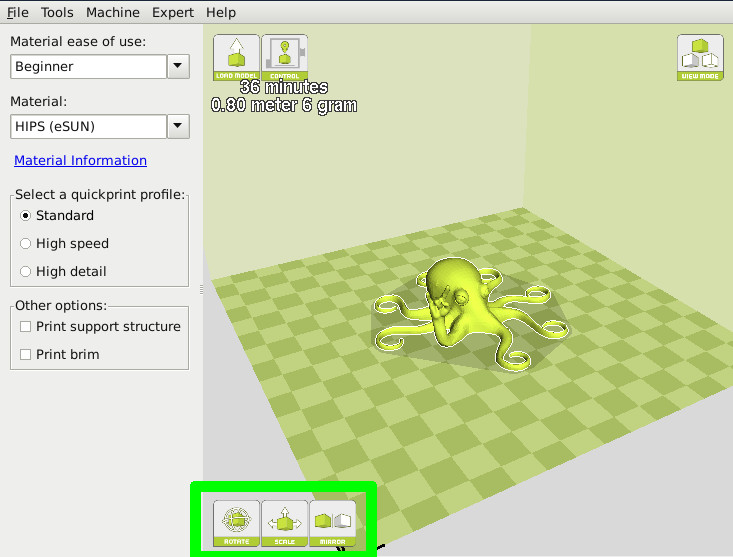
\includegraphics[keepaspectratio=true,angle=0,height=0.4\textheight,width=1.0\textwidth]{optionsRSM1.jpg}
\caption{Options after selecting model}
\label{fig:Orientation}
\end{figure}

\subsubsection{\texttt{Rotate}}
%%%% Alternate explanation %%%%
%The \texttt{Rotate} button will give you the ability orient your model in along all three axes. Once you click the rotate button, three circles will surround your model. The red circle will allow you to rotate in the XY plane. The Yellow circle will rotate in the XZ plane. The Green circle will rotate in the YZ plane.
\definecolor{yellow1}{cmyk}{0,0,1,0.30}
The \texttt{Rotate} button will give you the ability to orient your model in all three axes. Once you click the rotate button, three circles will surround your model. The \textcolor{red}{red circle} will allow you to rotate around the \textcolor{red}{Z axis}. The \textcolor{yellow1}{Yellow circle} will rotate around the \textcolor{yellow1}{Y axis}. The \textcolor{green}{Green circle} will rotate around the \textcolor{green}{X axis}.
\begin{figure}[H]
\centering
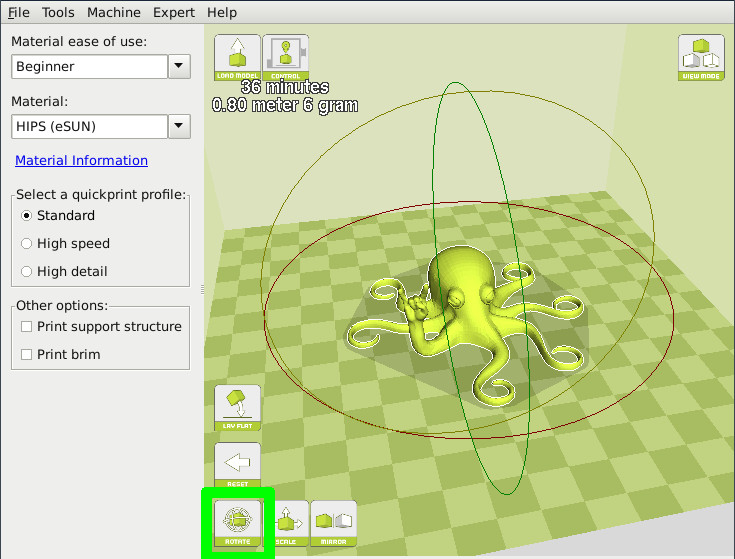
\includegraphics[keepaspectratio=true,angle=0,height=0.4\textheight,width=1.0\textwidth]{rotateoptions.jpg}
\caption{Rotating your Model}
\label{fig:Rotating your Model}
\end{figure}

\subsubsection{\texttt{Lay Flat}}
The \texttt{Lay Flat} button will ensure that the flat portion of your print is securely attached to the bed. It is highly recommended to use this option after rotating your model in the Z direction, as it will help prevent adhesion issues during the print.
%\begin{figure}[hbt]
%\centering
%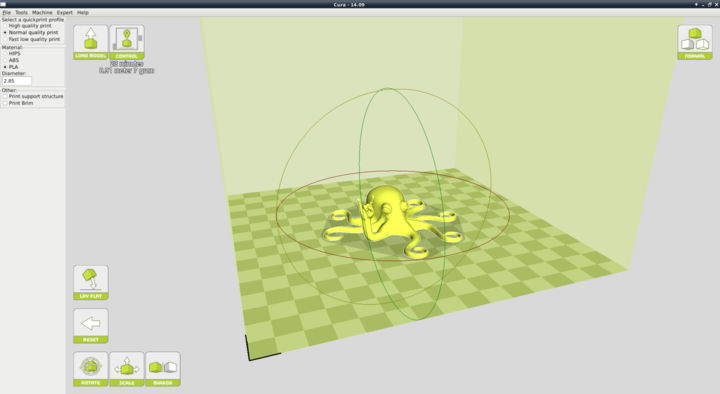
\includegraphics[keepaspectratio=true,angle=0,height=0.4\textheight,width=1.0\textwidth]{Rotate.png}
%\caption{Rotating your Model}
%\label{fig:Rotating your Model}
%\end{figure}

\subsubsection{\texttt{Reset}}
The \texttt{Reset} button will return your model to the original orientation as defined by the CAD program used to create the model.
%\begin{figure}[hbt]
%\centering
%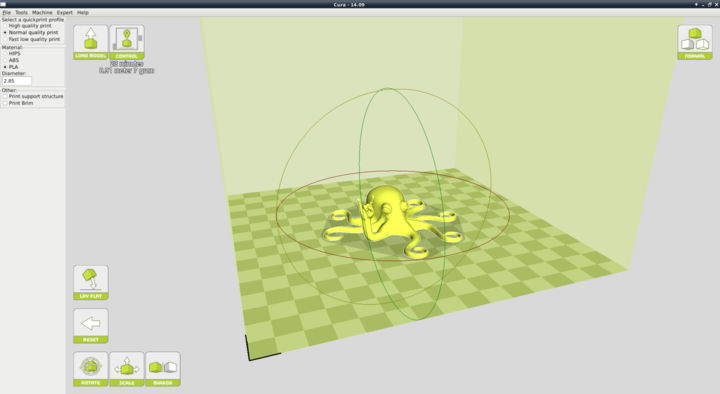
\includegraphics[keepaspectratio=true,angle=0,height=0.4\textheight,width=1.0\textwidth]{Rotate.png}
%\caption{Rotating your Model}
%\label{fig:Rotating your Model}
%\end{figure}

\subsubsection{\texttt{Scale}}
The \texttt{Scale} button displays the model dimensions, along with the ability to scale along the X Y or Z axes. Anything \texttt{below} the number \texttt{1.0} will reduce the objects size, while anything \texttt{above} the number \texttt{1.0} will increase the objects size. As a default, it will be set to uniform scaling. This will cause the X Y and Z axes to be scaled by the same amount when you make a change to any of them. To disable this, select the lock in the lower section of the scaling window. 
\begin{figure}[H]
\centering
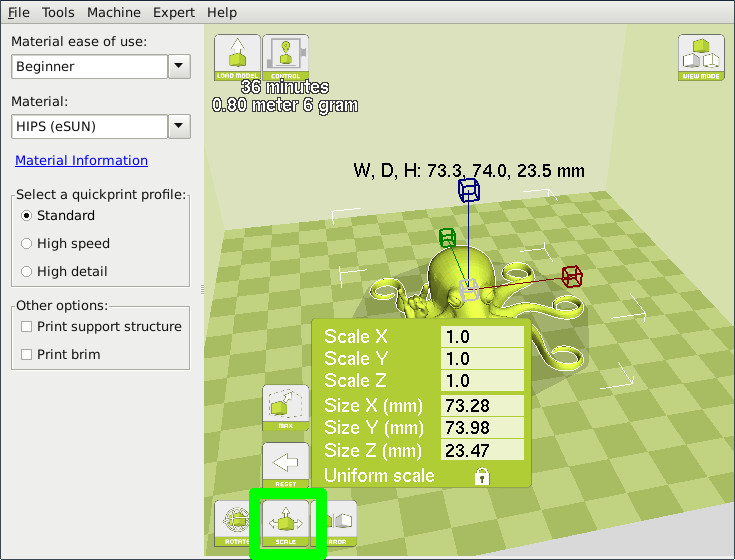
\includegraphics[keepaspectratio=true,angle=0,height=0.4\textheight,width=1.0\textwidth]{scaleoptions17.1.jpg}
\caption{Scaling your Model}
\label{fig:Scaling your Model}
\end{figure}

\section{\texttt{View Options}}
\index{View Options}
This mode allows you to view your model in a variety of different ways. This can be helpful for spotting issues before the print even starts. 

\subsection{\texttt{Normal}}
This is the standard view and shows the solid outer surfaces of the model. (Fig. \ref{fig:Normal View}, page \pageref{fig:Normal View}): 

\begin{figure}[H]
\centering
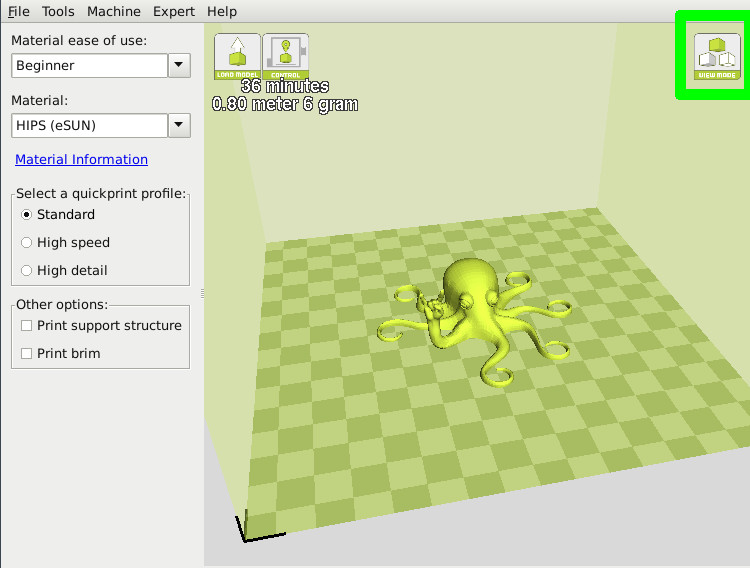
\includegraphics[keepaspectratio=true,angle=0,height=0.3\textheight,width=1.0\textwidth]{normalview17.1.jpg}
\caption{View in Normal Mode}
\label{fig:Normal View}
\end{figure}

\subsection{\texttt{Overhang}}
\index{Overhang} 
Overhang mode shows where your model may need support material. In Fig. \ref{fig:Overhang_View}, page \pageref{fig:Overhang_View} the red highlighted areas show overhangs and more severe angles and areas where support material is recommended.
\begin{figure}[H]
\centering
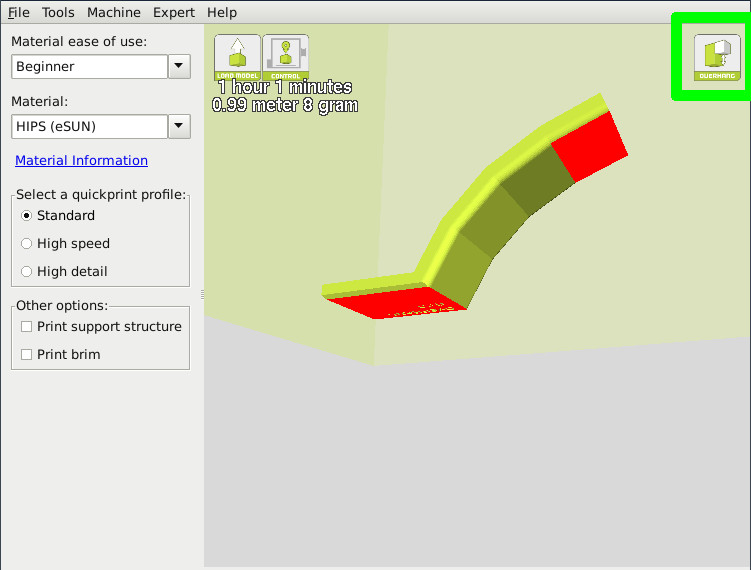
\includegraphics[keepaspectratio=true,angle=0,height=0.3\textheight,width=1.0\textwidth]{overhang17.1.jpg}
\caption{View in Overhang}
\label{fig:Overhang_View}
\end{figure}

\subsection{\texttt{Ghost}}
\index{Ghost}
Ghost view mode makes the model translucent to allow you to see what is behind it.
\begin{figure}[H]
\centering
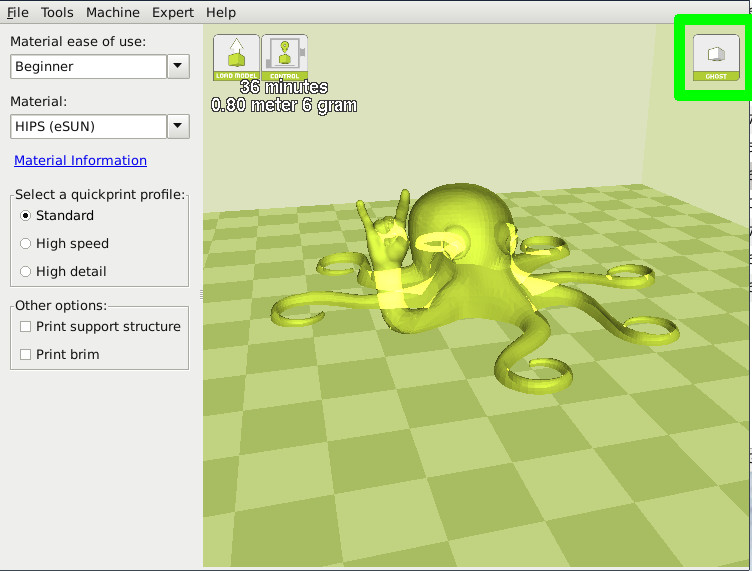
\includegraphics[keepaspectratio=true,angle=0,height=0.3\textheight,width=1.0\textwidth]{ghost17.1.jpg}
\caption{View in Ghost}
\label{fig:Ghost View}
\end{figure}

\subsection{\texttt{Xray}}
\index{Xray}
Xray is very similiar to Ghost mode. It will alow you to see into objects, ensuring that inner details are correct.
\begin{figure}[H]
\centering
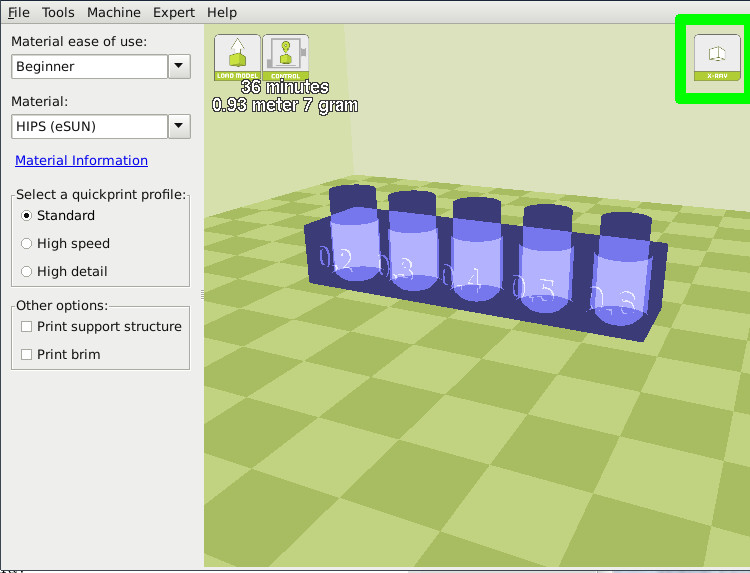
\includegraphics[keepaspectratio=true,angle=0,height=0.3\textheight,width=1.0\textwidth]{xray17.1.jpg}
\caption{View in Xray}
\label{fig:Xray View}
\end{figure}

\subsection{\texttt{Layers}}
\index{Layers}
To view the toolpath of your print head and to ensure no skipped layers or gaps use this option. Use the slide bar on the right hand side of the window to move up and down through the toolpath layers. The button just below the slide bar will toggle cumulative layers and individual layers.
\begin{figure}[H]
\centering
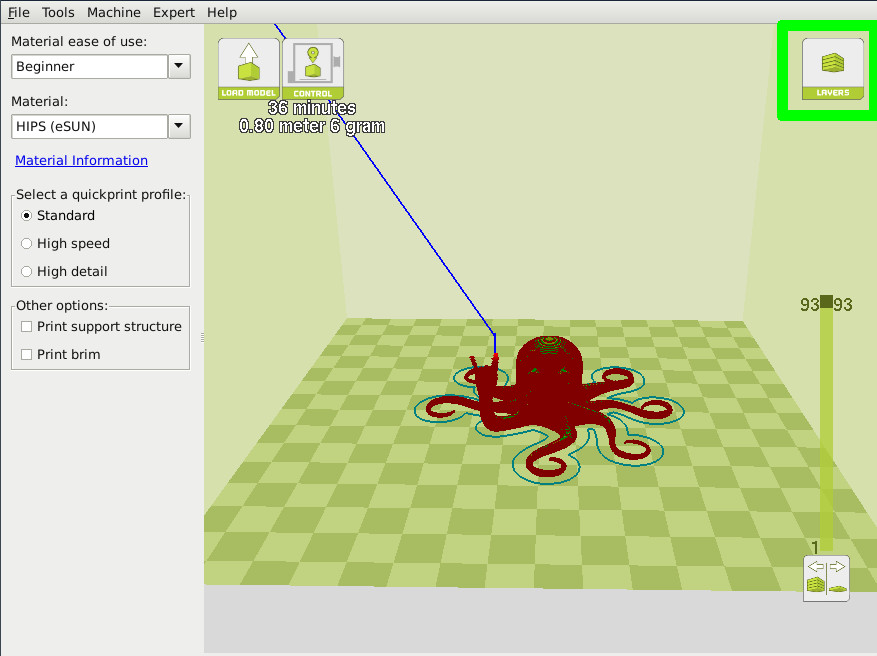
\includegraphics[keepaspectratio=true,angle=0,height=0.3\textheight,width=1.0\textwidth]{layers1.17.1.jpg}
\caption{View in Layers}
\label{fig:Layers View}
\end{figure}

\begin{figure}[H]
\centering
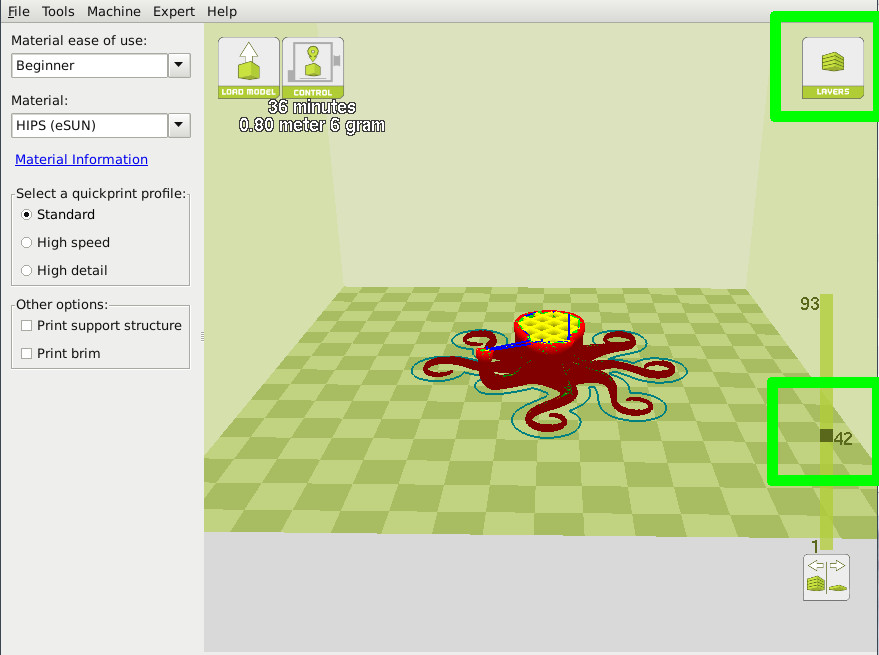
\includegraphics[keepaspectratio=true,angle=0,height=0.3\textheight,width=1.0\textwidth]{layers2.17.1.jpg}
\caption{Viewing Specific Layers}
\label{fig:Mid Layers View}
\end{figure}

\begin {figure}[H]
\centering
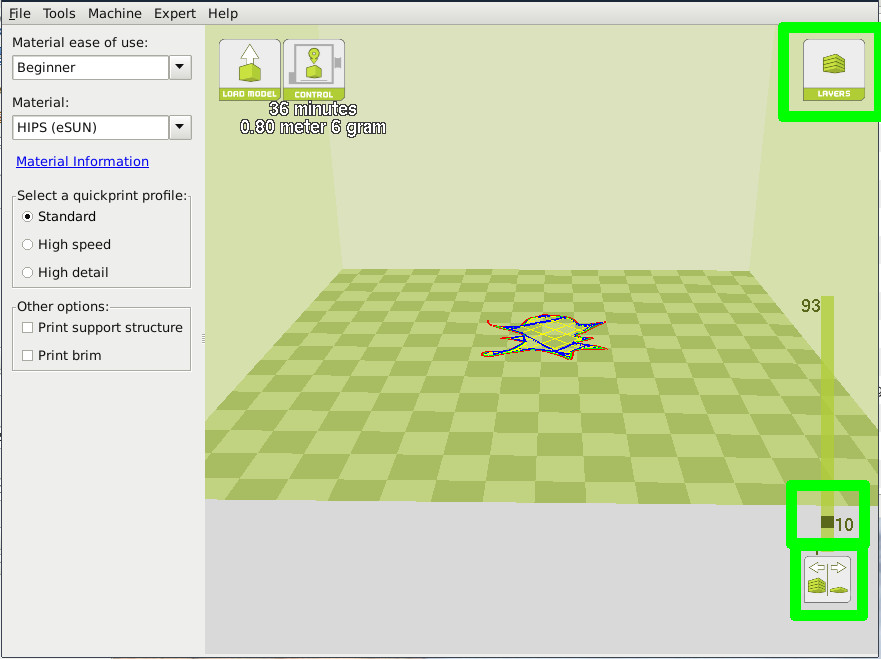
\includegraphics[keepaspectratio=true,angle=0,height=0.3\textheight,width=1.0\textwidth]{layers3.17.1.jpg}
\caption{Viewing Individual Layer}
\label{fig:Specific Layer}
\end{figure}

\section{\texttt{Starting Your First Print}}
\index{First Print}
Once you have your model, profile, and filament loaded, it is time for your first print! 

\begin{comment} %%%% Turn the following on for standalone Cura manual %%%%
\subsection{Mini}

Select the \texttt{Print/Control} option in the top left hand corner of your build volume. This will bring up your Pronterface user interface. Please wait for the window to state \texttt{operational} before sending any commands to the printer..

%\pageref{fig:Print Control}).
\begin{figure}[hbt]
\centering
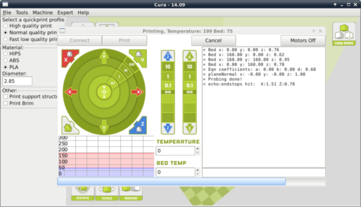
\includegraphics[keepaspectratio=true,angle=0,height=0.4\textheight,width=1.0\textwidth]{print_control.png}
\caption{Print Control Screen}
\label{fig:Print Control}
\end{figure}

\subsection{TAZ}

TAZ users will need to decide if they want to print directly from their computer using the USB cable, or if they would like to print from their SD card.

%%%% SD Printing %%%%
\subsubsection{Printing from SD Card}
\index{Printing from SD}

Save your Gcode file to your SD card. Select \texttt{File} > \texttt{Save Gcode} and choose the SD card location. Insert the SD Card into the Graphical LCD Controller.

\subsection{Set Temperature}

Turn on the heated bed and hot end by using the Graphical LCD controller and navigating to: \texttt{Prepare} > \texttt{Preheat ABS or PLA}. If you are using other materials you can set your desired temperatures by going to \texttt{Control} > \texttt{Temperature} > \texttt{Nozzle/Bed}. Wait for your 3D printer to reach specified temperatures.

\subsection{Start Print}
\index{printing}
Once at the desired printing temperature begin your print through your Graphical LCD controller by navigating to: \texttt{Print From SD} > and select the desired file.

%%%% Tethered printing %%%%

\subsubsection{Printing from USB Cable}
\index{Printing from USB}

Connect your 3D printer using a USB cable and select the \texttt{Print/Control} button. This will bring up the Pronterface user interface. You will not be able to send any commands until the window title changes to \texttt{Operational}. 

\subsubsection{Set Temperature}

Set your temperatures for the hot end and the bed. You will see two boxes, one labeled “Temperature” and one labeled “Bed Temp”. Temperature will set your hot end, and bed temp will set your bed. Once your hot end and bed have reached temperature, you will just need to select print.

\end{comment} 

\subsection{\texttt{Control}}
\index{Control}
Connect your 3D printer to a computer using a USB cable, and power it on and select the \texttt{Control} button. \texttt{You must have an STL file loaded in order for the control button to appear.}  This will bring up your Pronterface user interface. You will not be able to send any commands until the window title changes to \texttt{Operational}. As soon as it is operational, select \texttt{Print}. This will start the printing process: (set the appropriate temperatures, go through the auto-leveling procedure, and start printing your model). \textcolor{red}{Watch your automatic bed leveling sequence every print.} If your nozzle bends down your corner washers, turn off the printers power and restart the print.
%\pageref{fig:Print Control}).
\begin{figure}[H]
\centering
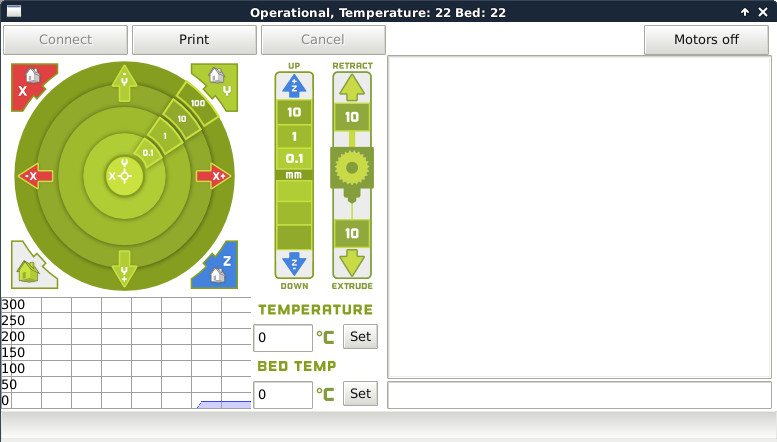
\includegraphics[keepaspectratio=true,angle=0,height=0.4\textheight,width=1.0\textwidth]{ControlBox17.1.jpg}
\caption{Control Screen}
\label{fig:Control}
\end{figure}
\subsection{\texttt{Pausing Mid-Print}}
\index{Pause}
You will notice after you click the print button through Cura, it will change to a pause button. When activated, it will pause your print and automatically move your print head away from your object. This will allow color changes or material changes mid print.
\subsection{\texttt{Recommended Temperatures}}
\index{Temperatures}
Different filaments have different ideal temperatures for extrusion, bed adhesion, and part removal. Your LulzBot Mini will have these automatically set when using our recommended profiles. We have found that for certain materials a glue stick is required for successful bed adhesion and/or part release. Glue stick can also be added to help first layer adhesion on any material, and may be helpful for objects with a larger surface area. 
\begin{center}
 \hspace*{-1.5cm}\begin{tabular}{||c c c c c||} 
 \hline
 Filament Type & Bed Preparation & Nozzle Temp & Bed Temp & Removal Temp \\ [0.5ex] 
 \hline\hline
 ABS & Clean PEI & 240-260 & 110 & 50 \\ 
 \hline
 PLA & Clean PEI & 195-215 & 60 & 45 \\
 \hline
 HIPS & Clean PEI & 240-260 & 110 & 50\\
 \hline
 Laywoo-D3 & Clean PEI & 175-195 & 60 & 45 \\
 \hline
 Laybrick & Clean PEI & 175-195 & 60 & 45 \\
 \hline 
 Magnetic Iron PLA & Clean PEI & 220-230 & 60 & 45 \\
 \hline
 Stainless Steel PLA & Clean PEI & 220-230 & 60 & 45 \\
 \hline
 Conductive PLA & Clean PEI & 215-230 & 60 & 50 \\
 \hline
 nGen & Clean PEI & 225-250 & 75 & 60 \\
 \hline
 t-glase & Glue stick & 240-260 & 60 & 45 \\
 \hline
 Flexible Filaments & Glue stick & 215-230 & 50 & 35 \\  
 \hline
 Nylons & Glue stick & 220-270 & 110 & 50 \\
 \hline
 Polycarbonate & Glue stick & 260-300 & 110 & 50 \\ 
 \hline
 Polycarbonate + ABS & Glue stick & 260-280 & 110 & 50 \\
 \hline
 INOVA 1800 & Glue stick & 235-255 & 75 & 50 \\
 \hline 
 n-vent & Glue stick & 220-260 & 110 & 50 \\ [1ex]
 \hline
 
\end{tabular}
\end{center}

\section{\texttt{Removing Your First Print}}
\index{Removing a Print}
After your first print has finished, you need to wait for the part to cool down.  Your parts will be easier to remove if you allow your heated bed to cool down to optimal temperature. This will allow the plastic to contract, making it easier to remove. \texttt{Your print bed will move forward once it is ready to be removed.}

Once your heated bed has cooled, use the blue handled knife that was included with your printer to remove the item. Carefully insert the blade of the knife between your print and heated bed. Once underneath the part rotate the blade- lifting with the sharp edge into the part, to gently pop the piece off your plate.
%\begin{figure}[hbt]
%\centering
%\includegraphics[keepaspectratio=true,angle=0,height=0.4\textheight,width=1.0\textwidth]{remove_part.png} %%%% Photo needed %%%%
%\caption{Remove Part}
%\label{fig:Remove part}
%\end{figure}

\section{\texttt{Full Settings}}
\index{Full Settings}
\textcolor{red}{When switching to full settings, it is important to transfer over a filament specific profile.} Your LulzBot Mini Operates on filament specific profiles, and if you do not transfer over the settings your Mini will not function as intended. 
The first time Cura is launched it will default to the \texttt{Quick Print} interface. In order to have more control of your slicing and Gcode generation, switch to \texttt{Full Settings}. First, select your intended filament and desired resolution. Then, Select \texttt{Expert} > \texttt{Switch to full settings}. Be sure to select \texttt{Yes} when prompted.
\begin{figure}[H]
\centering
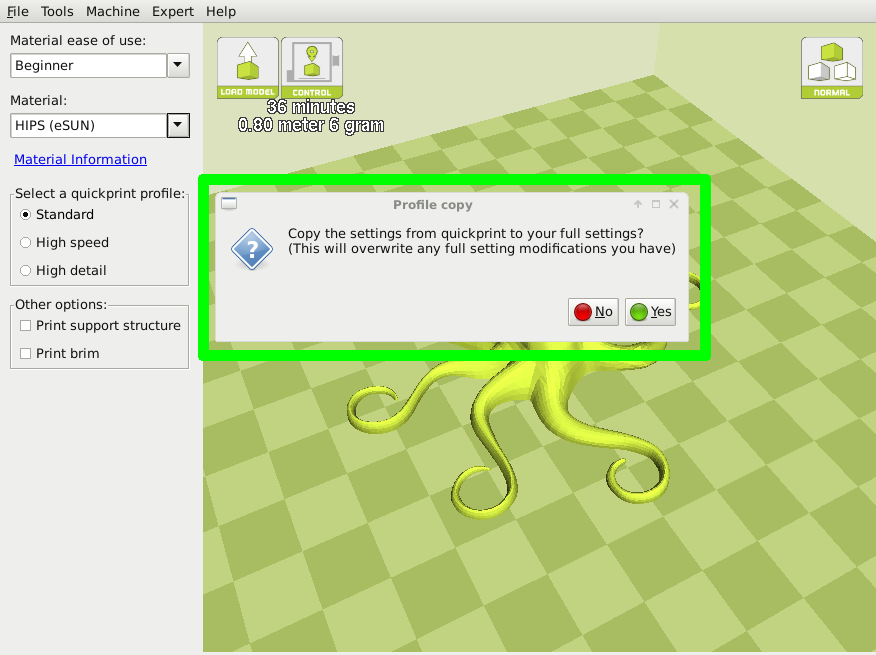
\includegraphics[keepaspectratio=true,angle=0,height=0.4\textheight,width=1.0\textwidth]{copyprofile.jpg}
\caption{Transferring a Profile}
\label{fig:Transferring a Profile}
\end{figure}
Once the switch has been made to full settings, you will now have access to a wide variety of options. You will notice 4 new tabs: \texttt{Basic, Advanced, Plugins, Start/End-Gcode}. In the following sections we will describe each option, and how they will affect your prints.
\begin{figure}[H]
\centering
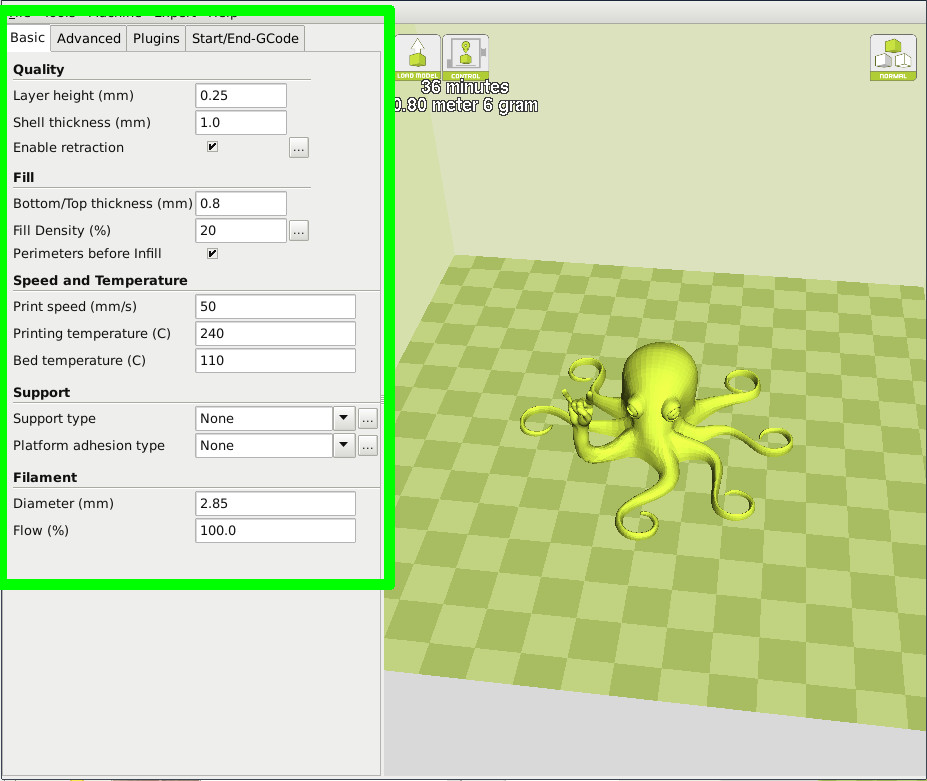
\includegraphics[keepaspectratio=true,angle=0,height=0.4\textheight,width=1.0\textwidth]{fullsettings17.1.jpg}
\caption{View in Full Settings}
\label{fig:View in Full Settings}
\end{figure}

\subsection{\texttt{Loading a Profile}}
\index{Loading Profile}
Profiles determine how Cura turns your STL file into Gcode that controls your printer. Different filaments require different settings for optimal performance. As new filaments are being developed every day, there may be a time you need to manually load a profile. You can download our recommend profiles at: \texttt{https://www.lulzbot.com/support/mini-cura-profiles}. Once downloaded, load the filament specific .ini file by going to \texttt{File > Open Profile}.
%\begin{figure}[hbt]
%\centering
%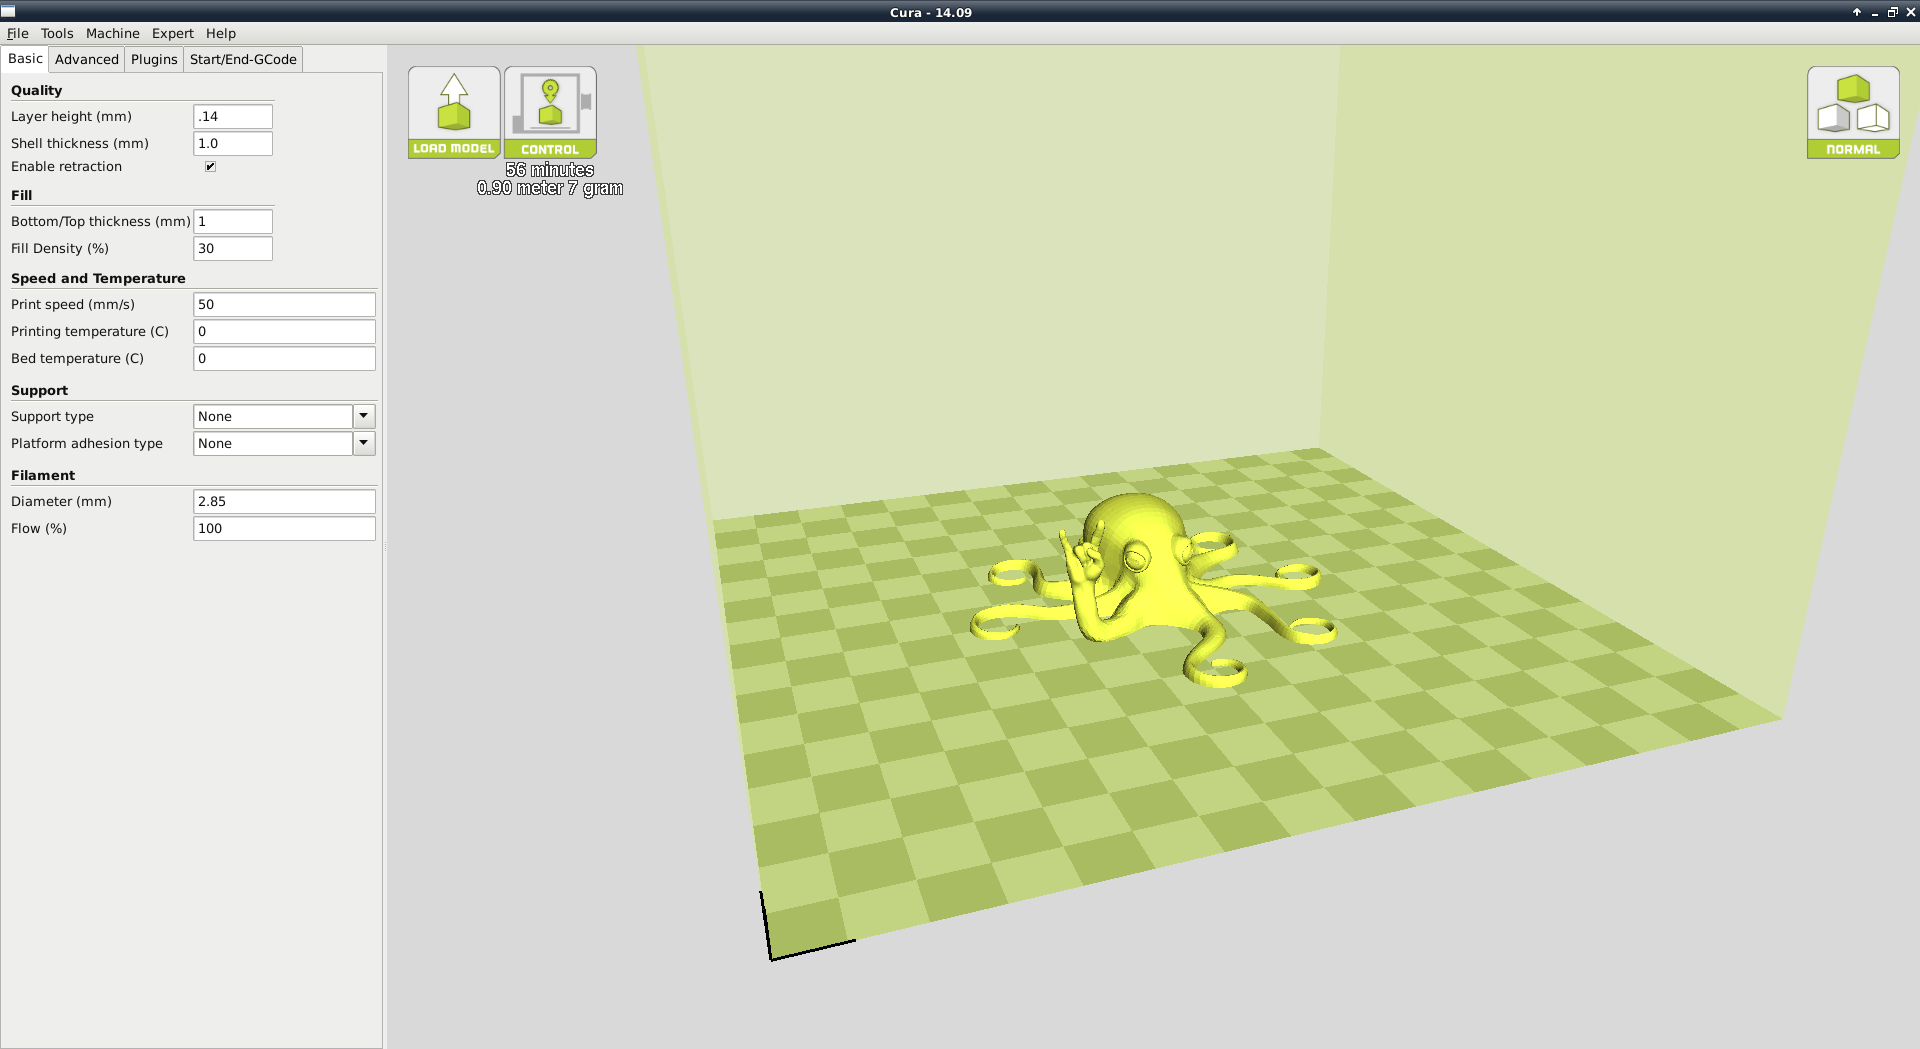
\includegraphics[keepaspectratio=true,angle=0,height=0.4\textheight,width=1.0\textwidth]{Expert.png}
%\caption{View in Full Settings}
%\label{fig:Full Settings View}
%\end{figure}

\section{\texttt{Basic Tab Options}}
\index{Basic Options}

\subsubsection{\texttt{Layer Height}}
\index{Layer Height}
The thickness of each printed layer is known as the \texttt{Layer Height}. The smaller the layer height, the smoother curves will appear. Larger layer heights are better for bridging and overhangs. Smaller layer heights will also increase print time, as it will take more layers to complete the object.
% (Layer height comparision photos)
\begin{figure}[H]
\centering
\includegraphics[keepaspectratio=true,angle=0,height=0.4\textheight,width=1.0\textwidth]{Layer_Height1.jpg}
\caption{Differences in Layer Height}
\label{fig:Differences in Layer Height}
\end{figure}


\subsubsection{\texttt{Shell Thickness}}
\index{Shell Thickness}
This defines the number of vertical walls that comprise the outside of your model. We recommend keeping this set to multiples of your nozzle width. Your LulzBot Mini 3D printer is equipped with a 0.5 mm nozzle. %The TAZ ships with a .35mm nozzle standard, while the TAZ Mini has a .5mm nozzle standard.

\subsubsection{\texttt{Enable Retraction}}
\index{Retraction}
Retraction tells your printer to pull filament out of the hot end upon travel moves. Travel moves are when your print head moves from one area of the print, to another without laying down filament. We recommend keeping this on for all filament types, and adjusting the retraction length and speed for the specific filament.
%(Details given in advanced tab section. ((Reference?))

\subsubsection{\texttt{Bottom/Top Thickness (mm)}}
\index{Bottom Thickness}
\index{Top Thickness}
Also known as \texttt{Surface Layers}- this will determine how thick the top and bottom layers are. A larger number here will create a thicker top and bottom which can be helpful for strength, bridging, and quality purposes. We recommend keeping this number as a multiple of your layer height.

\subsubsection{\texttt{Fill Density}}
\index{Fill Density}
This number is expressed as a percentage. 0\% will give a completely hollow print, while 100\% will give you a completely solid object. We have found that 20\% to 40\% fill density is functional for most prints.

\subsubsection{\texttt{Print Speed (mm/s)}}
\index{Print Speed}
Your overall printing speed can be adjusted here. If no other speeds are determined in the later sections your printer will automatically default to this speed. This speed will be different, depending on what type of filament you are using.

\subsubsection{\texttt{Printing Temperature}}
\index{Printing Temperature}
When using different filament materials you'll need to update the desired hot end and heated bed temperature. Any temperatures specified here will be used to automatically set both the hot end and heated bed. Your print will not begin until these temperatures are met. The Mini 3D printer needs to have the temperature specified in order to run through the automatic bed-leveling routine.
%%%% Since the Mini needs to have gcode temps set in order to run through auto bed leveling, the following statement is only applicable to the TAZ4 or earlier. %%%%
%We recommend leaving this temperature setting to “0”. If you set your temperature in this section your printer will not begin printing until it reaches the specified temperature. We recommend setting your printing temperatures through the Pronterface UI, or through your LCD.

\subsection{\texttt{Support Type}}
\index{Support Type}
Some models will require support material in order to print properly. This will usually occur when an object has an angle in relation to the build plate between 0 to 45 degrees. It is highly recommended to orient your object so that it minimizes or eliminates the need for support.

\subsubsection{\texttt{Touching Buildplate}}
This causes the support material to build up between the heated bed and the object. The red example is Touching Buildplate.
% (Photo of Circle inside a square, that is printed vertically. Have samples on photo table. Reference photo below?)

\subsubsection{\texttt{Everywhere}}
This prints support material between the heated bed and object as well as between the object and itself. The green example is Support Everywhere.
% (Photo of Circle inside a square, that is printed vertically, sample on photo table. Reference Photo Below?)
% (Support Comparison Photo)
\begin{figure}[H]
\centering
\includegraphics[keepaspectratio=true,angle=0,height=0.4\textheight,width=1.0\textwidth]{Support_Revised.jpg}
\caption{Support Types}
\label{fig:Different Types of Support}
\end{figure}

\subsection{\texttt{Platform Adhesion Type}}
\index{Adhesion Type}
Some models have a small surface area contacting the plate. This can create adhesion issues causing your part to pop off at some point during the print. To fix this, use either \texttt{Brim} or \texttt{Raft}. Raft is better used when a model has small heated bed contact points and overhangs.

\subsubsection{\texttt{Brim}}
\index{Brim}
Brim will create a single layer of filament, contacting and surrounding your model. This will increase the surface area of the part contacting the build platform thereby preventing it from popping off the heated bed. Brim will also help in situations where you are seeing corner lift. Brim settings can be adjusted in the \texttt{Expert Settings} options.
% (See Expert Settings/Page REFERENCE)

\subsubsection{\texttt{Raft}}
\index{Raft}
%% Raft is rarely used these days %%
Raft will generate a layer of material underneath your object. Raft was more often used before the addition of heated plates to increase surface area. Raft settings can be adjusted in the \texttt{Expert Settings} options.

\subsection{\texttt{Filament Diameter}}
\index{Filament Diameter}
The filament diameter setting is one of the more important settings. Make sure that you update this value periodically with your average filament diameter. While your filament may be referred to as 3mm, it is more likely going to be near 2.9mm +/- 0.1mm. You will want this to be an accurate average, as it will allow your printer to correctly calculate how much filament it is pulling into the hot end.

\subsection{\texttt{Filament Flow \%}}
\index{Flow Rate}
This controls how much filament your printer is extruding in relation to speed. This setting is mainly used to adjust for filament density variations. Leave this value at 100\% as changing it can lead to surface quality issues.

\section{\texttt{Advanced Tab Options}}
\index{Advanced Options}
\begin{figure}[H]
\centering
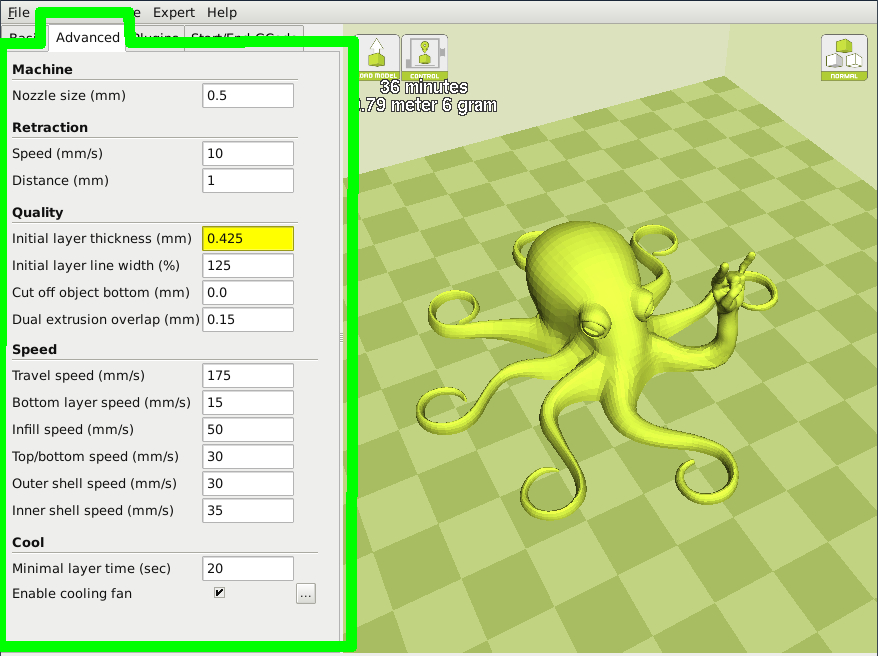
\includegraphics[keepaspectratio=true,angle=0,height=0.4\textheight,width=1.0\textwidth]{advanced.jpg}
\caption{View of Advanced Tab}
\label{fig:View of Advanced Tab}
\end{figure}

\subsection{\texttt{Nozzle Size (mm)}}
\index{Nozzle Size}
%%%% standalone version line %%%%
%This defines your nozzle size. The slicing engine uses this value combined with your other settings to determine how quickly to feed filament into your hot end. The TAZ ships with a 0.35mm nozzle, and the TAZ Mini ships with a 0.5mm nozzle.
This defines your nozzle size. The slicing engine uses this value combined with your other settings to determine how quickly to feed filament into your hot end. The Mini ships with a 0.5mm nozzle.

\subsection{\texttt{Retraction Speed (mm/s)}}
\index{Retraction Speed}
Retraction Speed determines the speed at which your filament is reversed out of the hot end for travel moves and when changing direction during printing. We recommend keeping this set to 25mm/s.

\subsection{\texttt{Retraction Distance}}
\index{Retraction Distance}
Retraction Distance determines how much filament is pulled out of your hot end on travel moves and when changing direction. You will want to adjust this depending on temperature settings and filament type. Higher thermal retaining filaments such as PLA behave better with a longer retraction distance. We have found anywhere from 1mm to 3mm is a good starting range.
% changed from "1 to 6mm" to remain conservative.

\subsection{\texttt{Initial Layer Thickness}}
\index{Initial Layer}
This will control how thick your first printed layer height is printed onto the heated bed. Having a larger initial layer height will help prevent your part from popping off the plate. \textcolor{red}{Your LulzBot Mini auto leveling system could be affected if you change this from the standard profiles. Adjust at your own risk.}
\subsection{\texttt{Initial Layer Line Width}}
\index{Initial Layer Width}
This will control how wide your first extruded filament path is for the initial layer. A wider line width will help with bed adhesion. We have found 125\% to be a good starting place. For models with moving printed in place parts, a smaller initial layer line width is recommended. \textcolor{red}{Your LulzBot Mini auto leveling system could be affected if you change this from the standard profiles. Adjust at your own risk.}

\subsection{\texttt{Cut Off Object Bottom (mm)}}
\index{Cut Off Object}
This setting is used to help print models that were not specifically designed for FFF printing. Specifically, it is for models that do not have a flat surface to adhere to the plate. It will sink your object Xmm into the build plate, creating a nice flat surface to begin your print. You can also use this option to remove the lower portion of your model.
\begin{figure}[H]
\centering
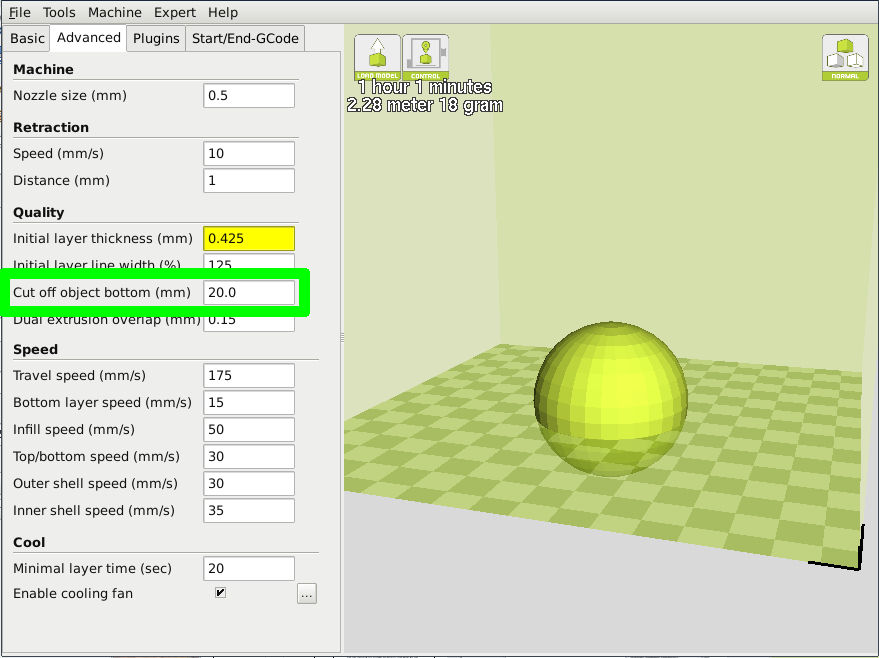
\includegraphics[keepaspectratio=true,angle=0,height=0.4\textheight,width=1.0\textwidth]{cutoff17.1.jpg}
\caption{Cutoff Example}
\label{fig:Cutoff Example}
\end{figure}

\subsection{\texttt{Dual Extrusion Overlap}}
\index{Dual Extrusion Overlap}
This will determine how far your Dual Extruders will overlap when laying down material. This will help adhesion between the two different colors or types of filament. This setting is only used when the printer is equipped with two hot ends and extruders.

\subsection{\texttt{Travel Speed}}
\index{Travel Speed}
This setting will determine how fast your print head moves while not extruding filament. A normal travel speed of 125 - 150mm/s is recommended.

\subsection{\texttt{Bottom Layer Speed}}
\index{Bottom Layer Speed}
This will control your initial layer speed. In general, a slower initial layer speed will help with first layer adhesion. 

\subsection{\texttt{Infill Speed}}
\index{Infill Speed}
This is how fast your print head speed will be while laying down the interior portion of your model. Faster speeds are usually tolerable here, as none of the infill will be visible from the outside of your object. If you go too fast compared to your inner and outer shells, you can have adhesion issues or globs of filament left behind from the printhead.

\subsection{\texttt{Outer Shell Speed}}
\index{Outer Shell Speed}
This will be the outermost surface of the model. This is the most important setting, as it controls the speed of your print head on the visible layers. As a general rule of thumb, the slower you go the better looking print you will get. 

\subsection{\texttt{Inner Shell Speed}}
\index{Inner Shell Speed}
This affects vertical walls that are in between the outer shell and infill. This will not be visible but will help support the outer shell and the infill. We recommend keeping this speed setting between your infill and your outer shell speed.

\subsection{\texttt{Minimal Layer Time}}
\index{Minimal Layer Time}
This will determine a minimum amount of time your printer will spend laying down each layer. If your layer print time falls below this your printer will automatically slow down to reach this time before moving onto the next layer. Tweaking this can help get cleaner, crisper prints.

\subsection{\texttt{Enable Cooling Fan}}
\index{Enabling Cooling Fan}
Enables operation of your extruder's active cooling fan. The fan settings can be adjusted in the \texttt{Expert Settings} options.

\section{\texttt{Plugins}}
\index{Plugins}
Plugins are custom settings which will alter your print at specific points. The two that come pre-loaded with Cura are \texttt{Tweak at Z}, and \texttt{Pause at Height}. More plugins and information can be found here: \texttt{http://wiki.ultimaker.com/Category:CuraPlugin} To activate one of these highlight the desired plugin and click the drop-down arrow directly below the Plugins box. 
\begin{figure}[H]
\centering
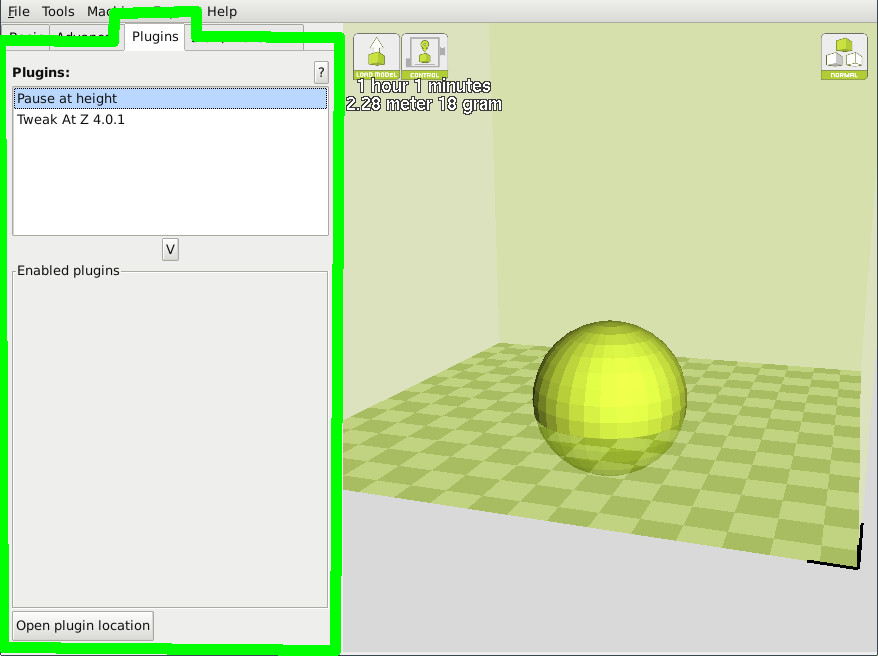
\includegraphics[keepaspectratio=true,angle=0,height=0.4\textheight,width=1.0\textwidth]{plugins17.1.jpg}
\caption{View of Plugins}
\label{fig:Plugins}
\end{figure}

\subsection{\texttt{Tweak at Z}}
\index{Tweak at Z}
Make basic changes at specified Z heights. You can determine the Z height or layer count at which you want to make a change. Then choose how you would like to change your settings. You can alter temperatures, fan speeds, and print speeds. Fine tuning these for specific STL files, can produce cleaner prints.

\subsection{\texttt{Pause at Z Height}}
\index{Pause at Z Height}
Pause your print at a specified height. You can also specify where to move the print head and how much filament to retract. This will prevent “blobs” from accumulating on your print while paused. This setting is most commonly used when switching colors of filaments in the middle of a print.

\section{\texttt{Start and End Gcode Settings}}
\index{Custom Gcode}
Custom Gcode allows for complex automatic printer movements and operations. By adding custom Gcode into the start or end of your file, you can alter how it prints. A comprehensive list of Gcode commands can be found here: \texttt{http://reprap.org/wiki/G-code} We recommend new users to leave this as provided in the profiles at \texttt{https://www.lulzbot.com/support/downloads}

\subsection{\texttt{Mini Specific Considerations}}
Please be cautious when changing any of these start and end gcode settings. \textcolor{red}{This is where your Auto Bed Leveling commands are stored. If improperly altered, your printer will no longer automatically compensate for the heated bed position and can even potentially damage components on the printer.} If you are uncertain of the change you are trying to make, please contact us at \texttt{Support@LulzBot.com} before hand.

\section{\texttt{Expert Settings}}
\index{Expert Settings}
Expert settings will give you more specific options for your retraction, skirt, active cooling, infill, support, brim, raft, and special settings. To gain access to this section you go to \texttt{Expert} > \texttt{Open Full Settings} or on your keyboard press \texttt{Control + E}.
\begin{figure}[H]
\centering
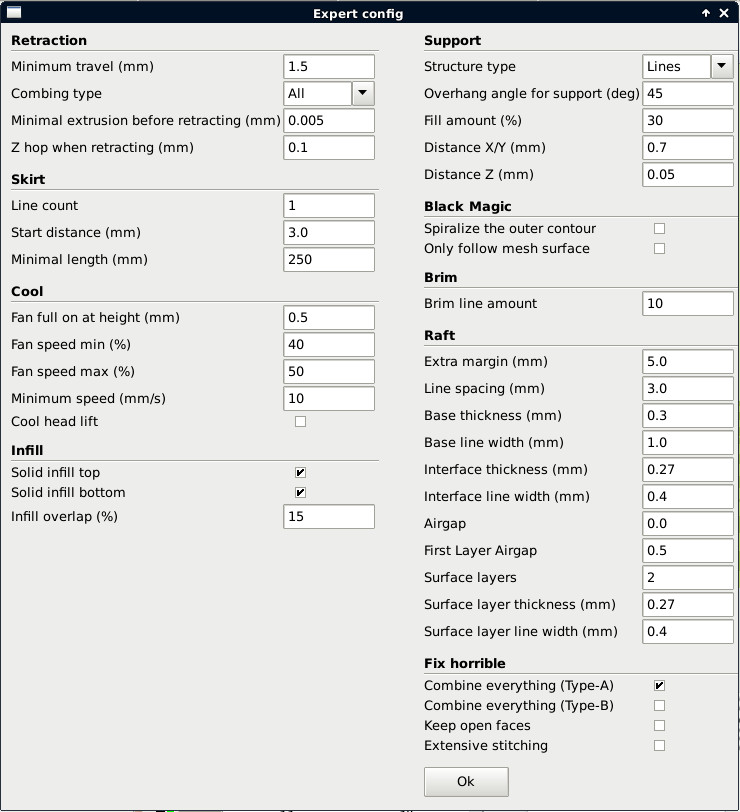
\includegraphics[keepaspectratio=true,angle=0,height=0.4\textheight,width=1.0\textwidth]{expert17.1.jpg}
\caption{View Expert Settings}
\label{fig:Expert Settings}
\end{figure}

\section{\texttt{Retraction}}
\index{Retraction}
Retraction pulls filament out of your nozzle when it is not extruding to prevent your print head from dripping on your object. This section is where you will control how your extruder retracts its filament.

\subsection{\texttt{Minimum Travel}}
\index{Minimum Travel}
This sets the minimum travel distance of your printhead in order to retract. If your print head is not moving this far during travel moves, it will not retract.

\subsection{\texttt{Combing}}
\index{Combing}
This option prevents your print head from traveling over holes in the X/Y plane when printing. This will slightly increase print time, but will prevent strings from getting caught on the holes during travel moves. We recommend keeping this setting on.

\subsection{\texttt{Minimal Extrusion Before Retracting}}
This will control the distance at which retraction occurs if the printing movement exceeds the minimum extrusion amount. This will prevent a retraction move, if your extruder has not put out Xmm of filament since its last retraction.

\subsection{\texttt{Z Hop When Retracting}}
\index{Z hop}
This will raise your print head Xmm while retracting. This setting helps prevent ooze, and strings from being deposited on your print. 
%\textcolor{red}{We do not recommend this setting for TAZ 3 users and earlier. This can cause issues with Z dimensional accuracy.}

\section{\texttt{Skirt}}
\index{Skirt}
Skirt creates a line around the outside of your object. Most commonly used to prime the extruder, in order to prevent missed filament at the beginning of a print. Leave this setting on.

\subsection{\texttt{Line Count}}
\index{Line Count}
This will define the number of loops the Skirt creates around the outside of your object. Smaller models will require more loops to properly prime the extruder.

\subsection{\texttt{Start Distance}}
\index{Start Distance}
This will define the distance away from your model that the skirt will be created. If using as an envelope to prevent drafts, it is recommended to be closer to your object.

\subsection{\texttt{Minimal Length}}
\index{Minmal Length}
This will define the minimum extruded line length for the skirt. This will over ride your line count, producing as many lines as required to reach the minimal length.

\section{\texttt{Cool}}
\index{Cooling}
This section will define how your extruder cooling fan will operate during the print. \textcolor{red}{Your fan will not start until it has reached 25\% or higher for speed settings.} If your print speeds are slowed down due to minimal layer time, the fan will run between minimum and maximum speed based upon how much the layer is slowed down.

\subsection{\texttt{Fan on at Full Height}}
\index{Fan Settings}
This is your Z height where your fan will be turned on to its minimum percentage setting. Especially helpful with high temperature retaining filaments such as PLA. This will be scaled between 0\%, and your minimum fan speed based upon layer height; with it being disabled for the first layer.

\subsection{\texttt{Fan Speed Min}}
\index{Fan Settings}

This will be the speed your fan runs when enabled at full height. Once the Z height is reached for Fan on at Full Height, this will be the speed your fan runs at.

\subsection{\texttt{Fan Speed Max}}
\index{Fan Settings}
This is the fastest speed at which your fan will ever run. When your print speed is slowed down due to minimal layer time, your fan will run between minimum and maximum speed. The maximum fan speed is reached when your printer must be slowed by 50\% or greater.

\section{\texttt{Support}}
\index{Support Material}
You define how your support material is generated here. You must have some form of support turned on in the basic settings in order for these settings to have an effect.

\subsection{\texttt{Structure Type}}
\index{Support Settings}
You can choose between a Grid or a Line pattern for your support material. The grid will be a checkerboard pattern in the X and Y direction. The line option will produce lines in along the y axis for support. The grid will provide stronger support than the line option, but will be harder to remove.

\subsection{\texttt{Overhang Angle for Support}}
\index{Overhang Angle}
This will determine where support material is generated. In general you will be able to print a model with 45 to 90 degree angles in relation to the bed without support. We recommend leaving this setting at 45.

\subsection{\texttt{Fill Amount}}
\index{Fill Amount}
This will determine how dense your support material is printed, similar to Infill Percentage. The higher percentage the better support, but it will be harder to remove the support material and will use more material.

\subsection{\texttt{Distance X/Y}}
\index{Support}
This will determine how far away from your object in the X/Y plane that the support material is being placed.

\subsection{\texttt{Distance Z}}
\index{Support}
This will determine how far away your support material is from your object in the vertical direction. A smaller number here makes for better support, but makes it harder to remove.

\section{\texttt{Black Magic}}
\index{Black Magic}
This section allows you to transform your model into a hollow shell, a single layer thick.

\subsection{\texttt{Spiralize the Outer Contour}}
\index{Spiralize}
This causes your Z axis to be constantly moving upward as printing your single outer wall shell. The results are no layer change lines, giving a much smoother surface. This setting is typically only used for artistic objects as they will be fragile.

\subsection{\texttt{Only Follow Mesh Surface}}
\index{Follow Mesh Surface}
This will cause your print to follow the outside of your model, building it completely hollow with a single wall outer shell. The only difference between this and Spiralize, is that the Z axis moves regularly. That is, it prints a layer and then moves up to the next one.

\section{\texttt{Brim}}
\index{Brim}
Brim circles the base of the print while making contact, helping adhere the print to the heated plate. This is only one layer thick, and easily removed post-print. This section defines how the brim is formed when brim is activated in basic settings.

\subsection{\texttt{Brim Line Amount}}
This will determine the distance the brim will cover around the outside of your object. The more brim used, the better your part will adhere to the plate. 

\section{\texttt{Raft}}
\index{Raft}
Raft is a platform built underneath your object, designed to help adhesion and prevent warping. It will lay down support material, and then a platform on top of the supports. Your model will be built on top of this platform. The bottom surface of your printed part will not be as clean or as even when using this option. Raft is typically not recommended.

\subsection{\texttt{Extra Margin}}
\index{Extra Margin}
This determines the distance around the outside of your object that the raft is created. Can be helpful for ensuring no warping of the lower layers.

\subsection{\texttt{Line Spacing}}
\index{Line Spacing}
This will determine the spacing between “support” lines for the raft. A small spacing makes the support structures closer together improving strength of the raft, but uses more material.

\subsection{\texttt{Base Thickness}}
\index{Base Thickness}
This defines how thick your raft will be.

\subsection{\texttt{Base Line Width}}
\index{Base Line Width}
This will define how wide your “support” material is for the raft. This setting will determine how well the surface layers of the raft print.

\subsection{\texttt{Interface Thickness}}
\index{Interface Thickness}
This will determine how thick the surface layers of the raft are. The surface layers are the platform that is built upon the supports.

\subsection{\texttt{Interface Line Width}}
\index{Interface Line Width}
This will determine how wide the top layers of the platform will be. In general, you can keep this set to your nozzle size, as surface quality of the removable raft is not important.

\subsection{\texttt{Airgap}}
\index{Airgap}
This will define the distance between your raft and your print. A larger gap will make your part easier to remove, but will make the bottom of your print look worse.

\subsection{\texttt{Surface Layers}}
\index{Surface Layers}
This will determine the number of layers that create the “platform” of your raft. If you have a wide line spacing, you may want to increase this number to ensure a solid platform. 

\section{\texttt{Fix Horrible}}
\index{Fix Horrible}
These are some of the more advanced and experimental options. They are designed to help repair models with errors to make them suitable for 3D printing. They do not always work. Please be cautious when using these options as they can have unintended effects on your print quality.

\subsection{\texttt{Combine Everything (Type-A)}}
\index{Combine Type-A}
This will attempt to fix all external mesh errors, while keeping internal holes intact. This can accidentaly fill in intentional internal holes.

\subsection{\texttt{Combine Everything (Type-B)}}
\index{Combine Type-B}
This will ignore all internal holes of the model and only focus on the external holes. This is helpful when only the outside finish of the model is important.

\subsection{\texttt{Keep Open Faces}}
\index{Open Faces}
This will ignore all manifold errors in the object. It can create issues generating the Gcode as Cura does not know how to interpret the open holes. This option should only be used if you are sure that the holes in the mesh are intended. In general, you should not use this option. %Really. Don't.

\subsection{\texttt{Extensive Stiching}}
\index{Extensive Stiching}
This causes Cura to automatically add triangle meshes in an attempt to fix manifold errors. This algorithm will greatly increase Gcode generation time and may end up adding in un-intended meshes. It is recommended that you repair your model through Meshlab or your CAD program before attempting this option.
